%!TEX program = xelatex
\documentclass[xcolor=table]{beamer}
\usepackage{ctex}
\usepackage{longtable}
\usepackage{multicol}
\usepackage{multirow}
\usepackage{setspace}
\usepackage{graphicx,hyperref,url, materialbeamer}
\usepackage{braket}
%\usepackage{euler}
\usepackage{listings}


\graphicspath{ {./figs/images/} }
\setbeamercovered{transparent}
\lstdefinestyle{customsql}{
  belowcaptionskip=1\baselineskip,
  breaklines=true,
  xleftmargin=\parindent,
  language=SQL,
  showstringspaces=false,
  basicstyle=\footnotesize\ttfamily,
  keywordstyle=\bfseries\color{green!40!black},
  commentstyle=\itshape\color{purple!40!black},
  identifierstyle=\color{blue},
  stringstyle=\color{orange},
}
\lstset{escapechar=@,style=customsql}



\usefonttheme{professionalfonts} % using non standard fonts for beamer
%\usefonttheme{serif}

% The title of the presentation:
%  - first a short version which is visible at the bottom of each slide;
%  - second the full title shown on the title slide;
\title{治未病健康传播新路径探索}

% Optional: a subtitle to be dispalyed on the title slide
\subtitle{基于知信行框架下的数字化再设计}

% The author(s) of the presentation:
%  - again first a short version to be displayed at the bottom;
%  - next the full list of authors, which may include contact information;
\author{付裕刚}
  
%\titlegraphic{\includegraphics[width=\textwidth]{atac-logo}}

% The institute:
%  - to start the name of the university as displayed on the top of each slide
%    this can be adjusted such that you can also create a Dutch version
%  - next the institute information as displayed on the title slide
\institute{第一临床医学院\\南京中医药大学
}

% Add a date and possibly the name of the event to the slides
%  - again first a short version to be shown at the bottom of each slide
%  - second the full date and event name for the title slide
\date[\today]{
 \today}


\begin{document}

\begin{frame}
  \titlepage
\end{frame}


\section{治未病健康传播的困境}
\begin{frame}{健康传播}
\centering
\begin{itemize}
    \item 通过各种渠道,运用各种传播媒介和方法制作、传递、分享健康信息的过程
    \item 大众传播媒介和效果研究
    \item 旨在提升公民健康素养
\end{itemize}
\end{frame}
\begin{frame}{微信健康传播}
\begin{columns}
    \begin{column}{0.5\textwidth}
        \begin{block}{微信公众平台优点}
            \begin{itemize}
                \item 互联网健康传播主要阵地
                \item 用户基数大,平台活跃度高
                \item 有较完善的互动机制
            \end{itemize}
        \end{block}
    \end{column}
    \begin{column}{0.5\textwidth}
        \begin{figure}[h]
            
\includegraphics[scale=0.3]{weixin.jpg}
        \end{figure}
    \end{column}
\end{columns}
\end{frame}
\begin{frame}{微信健康传播}
\begin{columns}
\begin{column}{0.5\textwidth}
\begin{exampleblock}{健康热点}
    \begin{itemize}
        \item 活跃的公众号已经超过1000万,其中涉及健康传播的超过半数。
        \vfill
    \textbf{健康议题成为中国人日常生活最关心的议题之一。}
    \end{itemize}
\end{exampleblock}
\end{column}
\begin{column}{0.5\textwidth}

\begin{figure}[h]
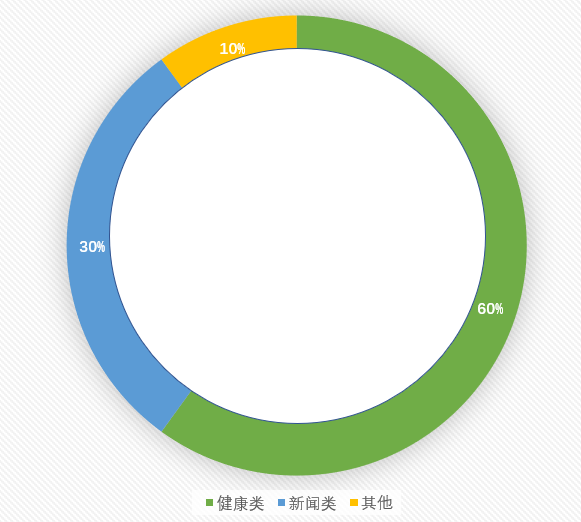
\includegraphics[scale=0.3]{zhanbi.png}
\end{figure}

\end{column}
\end{columns}
\end{frame}

\begin{frame}{微信健康传播}
\begin{columns}
    \begin{column}{0.5\textwidth}
        \begin{exampleblock}{传播内容}
            \begin{itemize}
                \item 传播内容重复,原创率低
                \item 权威中医内容少,术语化
                \item 存在大量灰色地带
            \end{itemize}
        \end{exampleblock}
    \end{column}
    \begin{column}{0.6\textwidth}
        
        \begin{figure}[h]
            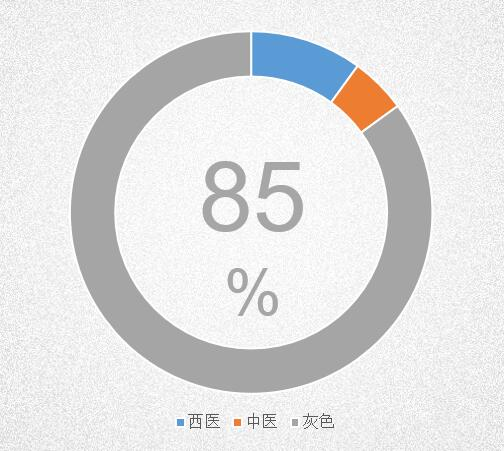
\includegraphics[scale=0.5]{content.jpg}
        \end{figure}
        
    \end{column}
\end{columns}
\end{frame}
%\begin{frame}{在“量大”的背后}
%\begin{columns}
%    \begin{column}{0.6\linewidth}
% 
%\begin{block}{传播乱象}
%尽管平台阅读量光鲜,但是内容质量低、缺乏体系、管理混乱的运营现状使得健康谣言激增,也使得互联网健康传播的可靠性受到诟病。健康传播的现状堪忧。
%\end{block}
%\end{column}
%\begin{column}{0.7\textwidth}
%    \begin{figure}[h]
%
\includegraphics[scale=0.4]{test}
%    \end{figure}
%\end{column}
%\end{columns}
%\end{frame}

\begin{frame}{政策背景}
\begin{columns}
    \begin{column}{0.5\textwidth}
       \begin{block}{发问}
       
           \vfill
           \begin{itemize}
               \item 什么样的知识信息是有效的?
               \item 怎么让治未病行为真正进入日常生活实践当中?
               \item 如何制定更好的治未病健康传播策略?
           \end{itemize}
       \end{block}
    \end{column}
    \begin{column}{0.5\textwidth}
\begin{block}{2018}
    《国务院办公厅关于促进“互联网+医疗健康”发展的意见》提出,建立网络科普平台,利用互联网提供健康科普知识精准教育,普及健康生活方式,提高居民自我健康管理能力和健康素养。
\end{block}
\end{column}
\end{columns}
\end{frame}

\begin{frame}{设想\&理论}
%\begin{block}{    发问}
%
%    \vfill
%    \begin{itemize}
%        \item 什么样的知识信息是有效的?
%        \item 怎么让治未病行为真正进入日常生活实践当中?
%        \item 如何制定更好的治未病健康传播策略?
%    \end{itemize}
%\end{block}
\large 建立大众喜闻乐见的数字平台进行治未病传播!
\vfill
\normalsize
 \begin{enumerate}
    \item 权威信息源头发布知识
    \item 受众接受知识,并反馈习得情况和态度
    \item 转化为正向行为
\end{enumerate}

\begin{block}{研究框架选择}
知信行理论模式是探究了知识、信念和行为三者之间联系的框架。知信行研究基于知识、信念、行为三个维度进行现状问卷调查,并加入实验干预。
\end{block}
\end{frame}
\begin{frame}{调研部分}
\begin{block}{调研目的}
基于知信行视角获知南京居民对中医药治未病的知晓度、信任度、依从度;同时了解居民和社区、社区医院的关系。
\end{block}
\begin{enumerate}
    \item 进行访谈
    \item 设计问卷题目
    \item 分析结论、展望
\end{enumerate}
\end{frame}
\section{调研部分报告}

\begin{frame}{角色的分化}
\begin{alertblock}{结论分述}
\begin{enumerate}
\item 居民:遇病求医现象突出;基于经济考虑,保健意识较薄弱

\item 社区医院:接待人群多为老人儿童;资金定额;治未病项目散列

\item 居委会:网格制度联系居民;治未病范畴宣教;慢病管理。
\end{enumerate}
\end{alertblock}
\begin{figure}[h]
    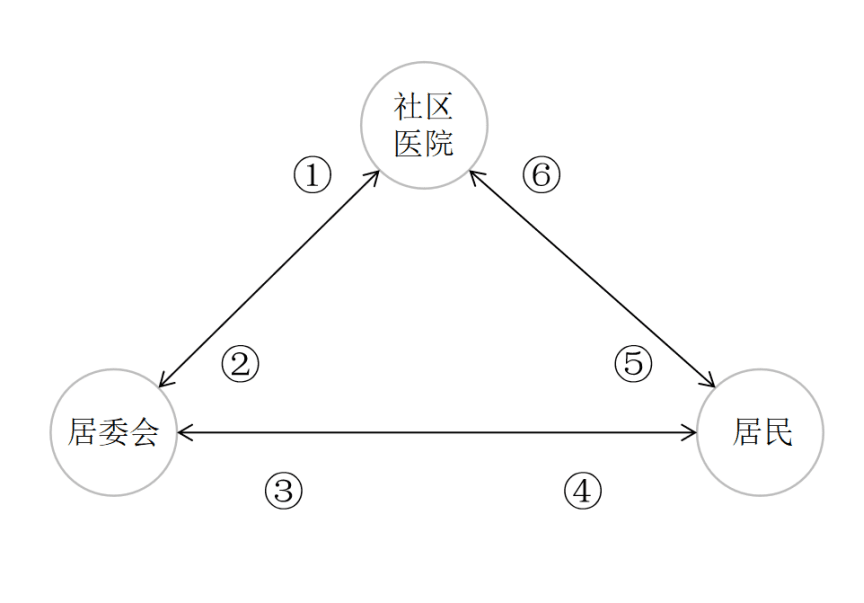
\includegraphics[scale=0.18]{guanxi.png}
    \centering
    \caption{互动关系说明}
\end{figure}
\end{frame}

\begin{frame}{定性结果分析}
通过定性访谈得出以下总体结论:
\begin{enumerate}
    \item 人群对于治未病知晓度尚可、信任度和依从度较低,和经济水平和观念意识相关。
    \item 治未病作为具体的实践项目在不同的机构扮演不同的角色,\textbf{在社区未能开展有效的治未病健康传播},需要另择他路。
\end{enumerate}
\end{frame}

\begin{frame}{问卷调查}
\begin{exampleblock}{调查目的}

\begin{enumerate}
    \item 居民治未病的知识、信念、行为情况的较普遍情况
    \item 上述情况和居民性别、年龄、教育、收入等的联系
\end{enumerate}\end{exampleblock}
\begin{alertblock}{方法}
    我们在南京市五福家园社区、东方城社区、兴隆社区、华侨路社区、凤凰二村社区发放先行设计的知信行问卷,共回收265份。统计分析如下:
\end{alertblock}
\end{frame}

\begin{frame}[allowframebreaks]{定量结果分析}
\begin{columns}
\begin{column}{0.7\textwidth}
    \begin{block}{各题维度、类型、跳题设置}
\begin{longtable}[]{@{}llll@{}}
    
    题号 & 维度 & 题目类型 & 是否有跳题\tabularnewline
    \hline
    \endhead
    1 & 知识 & 单选 & 是\tabularnewline
    2 & 知识 & 多选 & 否\tabularnewline
    3-10 & 知识 & 单选 & 否\tabularnewline
    11 & 知识 & 多选 & 否\tabularnewline
    12-19 & 信念 & 单选 & 否\tabularnewline
    20 & 行为 & 单选 & 是\tabularnewline
    21 & 行为 & 多选 & 否\tabularnewline
    22-26 & 行为 & 单选 & 否\tabularnewline
    \hline
\end{longtable}
\end{block}
\end{column}
\begin{column}{0.6\textwidth}
\begin{block}{分类变量}
\begin{longtable}[]{@{}lll@{}}
    
    题号 & 变量名称 & 类型\tabularnewline
    \hline
    \endhead
    27 & 性别 & 分类\tabularnewline
    28 & 年龄 & 数值\tabularnewline
    29 & 学历 & 分类\tabularnewline
    30 & 年收入 & 分类\tabularnewline
    \hline
\end{longtable}
\end{block}
\end{column}
\end{columns}
    \begin{columns}
    \begin{column}{0.6\textwidth}
\begin{figure}[h]\caption{居民治未病含义理解($N=122$)}
    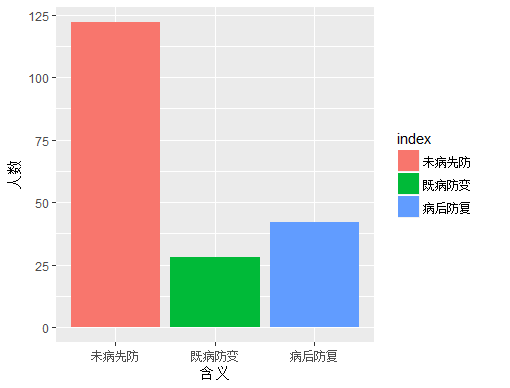
\includegraphics[scale=0.5]{./stats/hanyi.png}
    
\end{figure}
    \end{column}
    \begin{column}{0.6\textwidth}
        \begin{figure}[h] \caption{居民了解养生信息途径($N=265$)}
            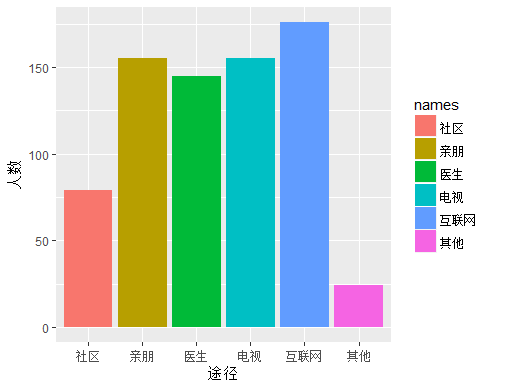
\includegraphics[scale=0.5]{./stats/ways.png}
           
        \end{figure} 
    \end{column}
\end{columns}

    \begin{columns}
    \begin{column}{0.5\textwidth}
        \begin{figure}[h]
            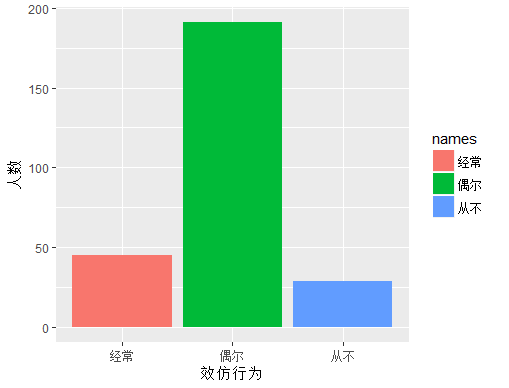
\includegraphics[scale=0.45]{./stats/zuofa.png}
            \caption{居民效仿养生做法频率}
        \end{figure}
    \end{column}
    \begin{column}{0.5\textwidth}
        \begin{figure}[h]
            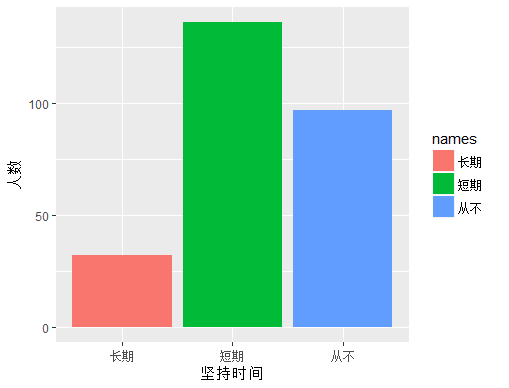
\includegraphics[scale=0.45]{./stats/jianchi.png}
            \caption{居民坚持养生做法时间}
        \end{figure} 
    \end{column}
\end{columns}


    \begin{columns}
    \begin{column}{0.5\textwidth}
        \begin{figure}[h]
            \caption{知识--态度--性别}
            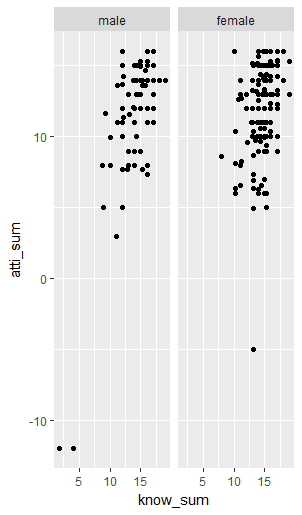
\includegraphics[scale=0.5]{./stats/know_sex.png}
            
        \end{figure}
           
    \end{column}
    \begin{column}{0.5\textwidth}
        \begin{figure}[h]
            \caption{知识--态度--收入}
           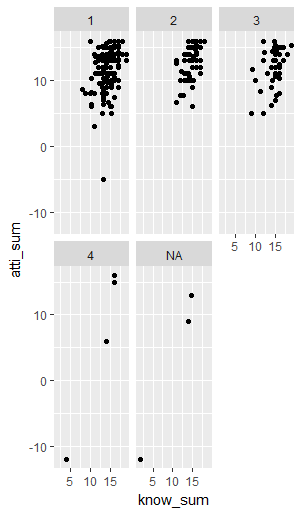
\includegraphics[scale=0.5]{./stats/know_income.png}
           
       \end{figure}
    \end{column}
\end{columns}

    \begin{columns}
    \begin{column}{0.5\textwidth}
        \begin{figure}[h]
             \caption{知识--态度--教育}
            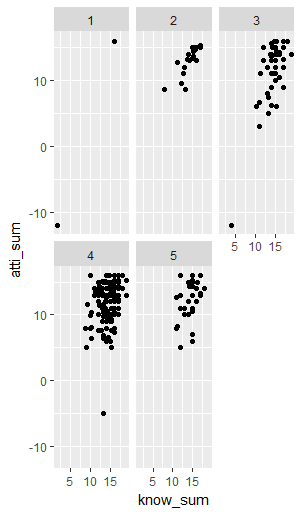
\includegraphics[scale=0.5]{./stats/know_grad.png}
           
        \end{figure}
        
    \end{column}
    \begin{column}{0.5\textwidth}
        \begin{figure}[h] 
            \caption{知识--态度--年龄}
            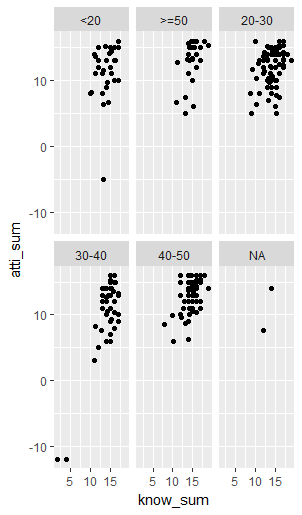
\includegraphics[scale=0.5]{./stats/know_age.png}
        \end{figure}
    \end{column}
\end{columns}

    \begin{columns}
    \begin{column}{0.5\textwidth}
        \begin{figure}[h]
            \caption{知识--行为--性别}
            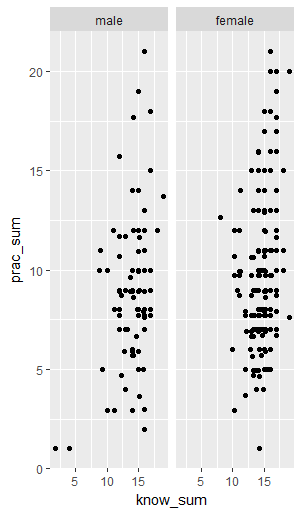
\includegraphics[scale=0.5]{./stats/prac_sex.png}
            
        \end{figure}
        
    \end{column}
    \begin{column}{0.5\textwidth}
        \begin{figure}[h]
            \caption{知识--行为--收入}
            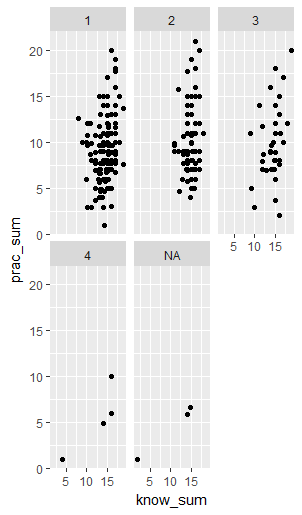
\includegraphics[scale=0.5]{./stats/prac_income.png}
            
        \end{figure}
    \end{column}
\end{columns}

    \begin{columns}
    \begin{column}{0.5\textwidth}
        \begin{figure}[h]
            \caption{知识--行为--教育}
            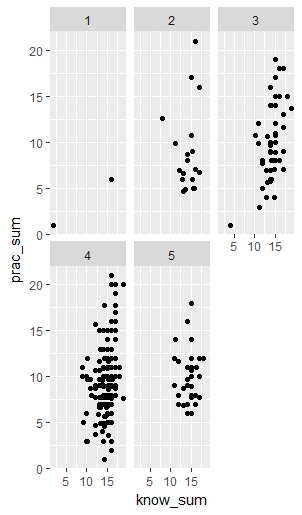
\includegraphics[scale=0.4]{./stats/prac_grad.png}
            
        \end{figure}
        
    \end{column}
    \begin{column}{0.5\textwidth}
        \begin{figure}[h] 
            \caption{知识--行为--年龄}
            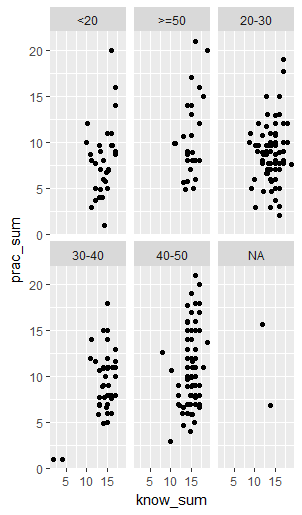
\includegraphics[scale=0.4]{./stats/prac_age.png}
        \end{figure}
    \end{column}
\end{columns}
    \begin{columns}
    \begin{column}{0.6\textwidth}
        \begin{figure}[h]
            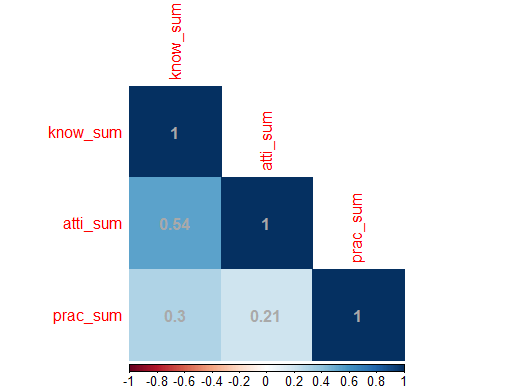
\includegraphics[scale=0.5]{./stats/corr.png}
            \caption{Pearson相关系数}
        \end{figure}
    \end{column}
    \begin{column}{0.6\textwidth}
        \begin{figure}[h]
            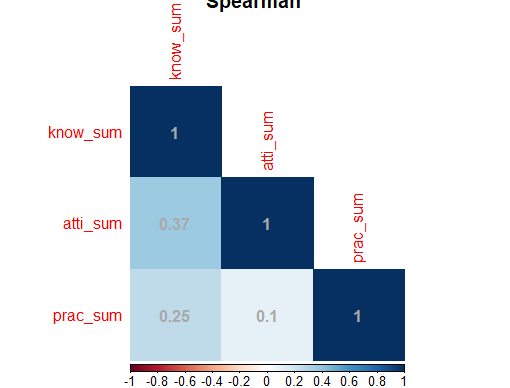
\includegraphics[scale=0.5]{./stats/cor_spearman.png}
            \caption{Spearman相关系数}
        \end{figure} 
    \end{column}
\end{columns}

\begin{exampleblock}{信而不行的原因}
    \begin{enumerate}
        \item 可能部分受调查者身体健康,没有就医或者保健的行动欲望
        \item 受调查者认为平常获取的养生信息可信度不高,不付诸实际行动
        \item 受调查者意志力不高,无法执行养生做法
        %220名被调查效仿过养生做法,但坚持不久就放弃了。
    \end{enumerate}
\end{exampleblock}
\end{frame}
\section{干预平台设计}
\setbeamercolor{background canvas}{bg=matblue}
\setbeamercolor{normal text}{fg=white}
\begin{frame}[plain, b]

\centering
\huge \textcolor{white}{进一步实验}
\normalsize

\vspace*{\fill}


\end{frame}
\setbeamercolor{background canvas}{bg=white}
\setbeamercolor{normal text}{fg=black}

%\begin{frame}{干预部分}
%\begin{enumerate}
%    \item 招募实验人员
%    \item 进行随机化分组
%    \item 进行实验
%    \item 整理数据,分析结果
%\end{enumerate}
%\begin{figure}[th]
%    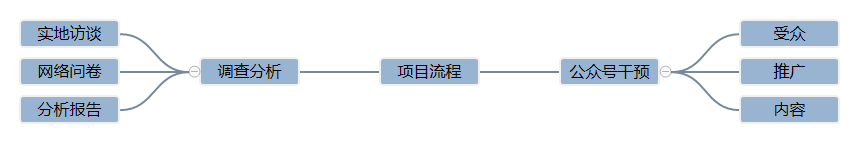
\includegraphics[width=\textwidth]{newprocess.png}
%    \centering
%    \caption{项目设计简图}
%\end{figure}
%\end{frame}
\begin{frame}{实验目的}
\begin{exampleblock}{实验目的}
    通过随机对照组实验尝试说明知识、信念、行为之间的转化关系,向治未病健康传播提供建议,并投入到已建成的平台上进行检验。
\end{exampleblock}
\begin{alertblock}{具体假设}
    
    \begin{enumerate}
        \item 经过知信行干预后各维度得分提高
        \item 同样强度的干预具有衰减效应,提高效果随时间推移减少
        \item 受监督组干预后得分较未监督组高
        \item 不同时间段阅读对干预效果无影响
    \end{enumerate}
\end{alertblock}

\end{frame}

\begin{frame}{既往研究}
\begin{columns}
    \begin{column}{0.4\textwidth}
   
\begin{block}{两个方向}
    \begin{itemize}
        \item 实验室环境对过程控制严格,自然环境相对松散
        \item 传统模式不使用数字化架构,数字模式则使用
    \end{itemize}
\end{block}
\end{column}
\begin{column}{0.6\textwidth}

\begin{figure}[h]
    \centering
    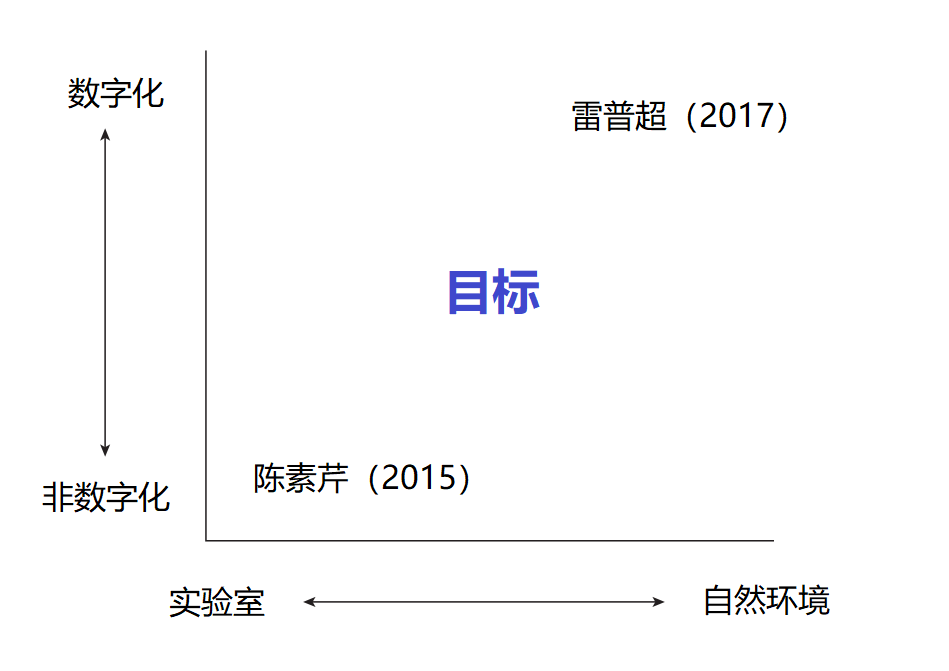
\includegraphics[scale=0.4]{digital.png}
    \caption{Adapted: Bit By Bit }
\end{figure}
\end{column}
\end{columns}
\end{frame}
\begin{frame}{既往研究}
\begin{columns}
    \begin{column}{0.4\textwidth}
\begin{exampleblock}{陈素芹2015}
    对肺病科住院的 100 例稳定期 COPD 进行知信行干预
    
    地点:医院
    
    方法:集体授课、一对一教育
    
\end{exampleblock}

\begin{exampleblock}{雷普超2017}
利用微信公众平台对大学生进行性教育知信行干预

地点:四川大学

方法:每周推送两篇科普短文、视频、书籍等
    
\end{exampleblock}
\end{column}
\begin{column}{0.6\textwidth}
    
    \begin{figure}[h]
        \centering
        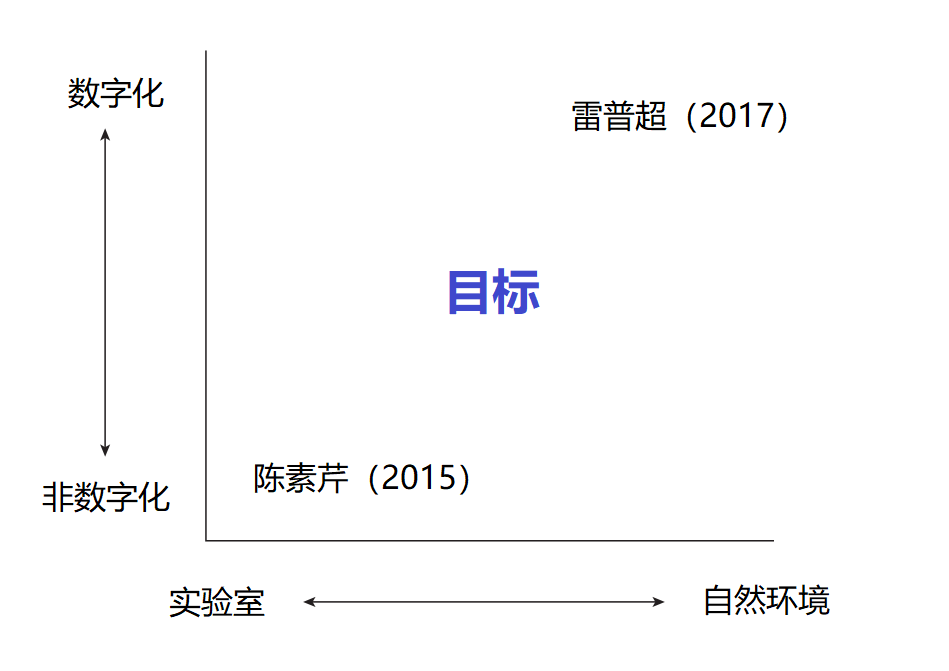
\includegraphics[scale=0.4]{digital.png}
        \caption{Adapted: Bit By Bit }
    \end{figure}
\end{column}
\end{columns}
\end{frame}



\begin{frame}{干预路径对比}
\begin{columns}
    \begin{column}{0.5\textwidth}
        \begin{block}{既往路径}
            \begin{itemize}
                \item 只进行了前测和终测
                \item 研究成本高,参与人数有限
                \item 对微信提供的功能利用不够
                \item 受干预时间和地点限制
            \end{itemize}
        \end{block}
    \end{column}
    \begin{column}{0.5\textwidth}
       \begin{block}{新路径}
          \begin{itemize}
              \item 通过标签/时间戳追踪,预测其中的衰减效应,阐释知信行变化机制
              \item 研究成本低,参与人数较多
              \item 更全面地利用微信提供的分析接口
              \item 打破时间和地点限制
          \end{itemize}
      \end{block}
    \end{column}
\end{columns}
\end{frame}

\begin{frame}{招募/实验平台选择}
\begin{columns}
    \begin{column}{0.5\textwidth}
\begin{block}{微信公众平台优点}
\begin{itemize}
    \item 使用基数大
    \item 研究成本低,开发便利,便于数据追踪和收集
    \item 数据更加真实,受调查者处于自然状态。
\end{itemize}
\end{block}
    \end{column}
\begin{column}{0.5\textwidth}
\begin{figure}[h]
    
\includegraphics[scale=0.3]{weixin.jpg}
\end{figure}
\end{column}
\end{columns}
\end{frame}

\begin{frame}{随机化\&实验分组}
\begin{enumerate}
    \item 随机数表进行分组
    \item 分为监督组(150)、非监督组(150)、对照组(150)
\end{enumerate}

\begin{block}{基于微信平台 特点}
    \begin{itemize}
        \item 投票功能:获得对监督组的反馈
        \item 图文分析:阅读量、阅读时间分布、终端
        
    \end{itemize}
\end{block}
\end{frame}



\begin{frame}{研究变量}
    \begin{itemize}
        \item 分类变量:性别、年龄、收入、教育水平、职业、婚姻状况、慢病情况
        \item 连续变量:知识、信念、行为三维度得分、健康水平(SF-36量表得分)
        \item 终端变量:地理位置、阅读量、时间戳
    \end{itemize}
\end{frame}


\begin{frame}{内容选择}
\begin{columns}
    \begin{column}{0.5\textwidth}
    \begin{block}{中医系列}
        \begin{itemize}
            \item 古人世界观、中医基本概念(30)
            \item 常见中药的介绍(20)
            \item 病案分析(15)
        \end{itemize}
    \end{block}
\end{column}
\begin{column}{0.5\textwidth}
    \begin{block}{养生系列}
        \begin{enumerate}
            \item 治未病饮食调理
            \item 治未病穴位保健
            \item 治未病运动功法
            \item 治未病精神调养
            \item 治未病热点专题
        \end{enumerate}
    \end{block}
\end{column}
\end{columns}
\end{frame}

\begin{frame}{平台预览}
    \begin{columns}
    \begin{column}{0.4\textwidth}
        \begin{figure}[h]
            
\includegraphics[scale=0.2]{wenzhang2.png}
            \caption{封面预览}
        \end{figure}
    \end{column}
    \begin{column}{0.4\textwidth}
        \begin{figure}[h]
            
\includegraphics[scale=0.2]{wenzhang.png}
            \caption{图文预览}
        \end{figure} 
    \end{column}
\begin{column}{0.4\textwidth}
           \begin{figure}[h]
       
\includegraphics[scale=0.2]{wenzhang3.png}
       \caption{图文预览}
   \end{figure} 
\end{column}
\end{columns}
\end{frame}

\setbeamercolor{background canvas}{bg=matblue}
\setbeamercolor{normal text}{fg=white}
\begin{frame}[plain, b]
\centering
\huge \textcolor{white}{谢谢您的聆听!}
\normalsize

\vspace*{\fill}


 \end{frame}

\end{document}
